\documentclass[../cours_tle.tex]{subfiles}
\begin{document}
\setcounter{chapter}{4}
\chapter{Vecteurs, bases et repères de l’espace}
\label{ch:5}
\begin{objectif}
Spécialité. Décrire des configurations en trois dimensions. Prérequis : vecteurs du plan et chapitre 1.
\end{objectif}
\section{Vecteurs et translations}
Un vecteur décrit un déplacement, indépendamment de son point de départ. La translation de vecteur $\vec u$ envoie $M$ sur l'unique $M'$ tel que $\overrightarrow{MM'}=\vec u$.
La relation de Chasles $\overrightarrow{AB}+\overrightarrow{BC}=\overrightarrow{AC}$ traduit deux déplacements successifs. Dans un repère, elle résulte aussi de $(B-A)+(C-B)=C-A$.
Une combinaison linéaire de $\vec u,\vec v,\vec w$ est $a\vec u+b\vec v+c\vec w$, avec $a,b,c\in\R$.
Deux vecteurs sont colinéaires si l'un est multiple de l'autre, avec le vecteur nul traité séparément ; une famille contenant le vecteur nul est dépendante.
\section{Décrire une droite et un plan}
\begin{definition}
La droite passant par $A$ de direction $\vec u\ne0$ est l'ensemble des $A+t\vec u$, $t\in\R$.
Le plan passant par $A$ de directions non colinéaires $\vec u,\vec v$ est l'ensemble des $A+s\vec u+t\vec v$, $(s,t)\in\R^2$.
\end{definition}
La notation $A+\vec u$ désigne le point obtenu par translation ; on n'additionne pas deux points sans avoir fixé une origine.
Trois vecteurs sont coplanaires s'ils appartiennent à un même plan vectoriel. Dans $\R^3$, trois vecteurs non coplanaires forment une base : chaque vecteur s'y écrit d'une manière unique.
\begin{demonstration}[Unicité des coordonnées]
Si $a\vec u+b\vec v+c\vec w=a'\vec u+b'\vec v+c'\vec w$, une différence non nulle entre les coefficients permettrait d'exprimer un des vecteurs comme combinaison des deux autres. Ils seraient coplanaires. Tous les coefficients sont donc égaux.
L'existence de la décomposition est le fait géométrique que trois directions non coplanaires engendrent l'espace ; le pivot du chapitre 32 en donne une lecture algébrique.
\end{demonstration}
Un repère associe une origine $O$ à une base. Les coordonnées d'un point $M$ sont celles de $\overrightarrow{OM}$ ; celles de $\overrightarrow{AB}$ sont $B-A$.
\section{Un cube pour voir les trois directions}
\begin{center}
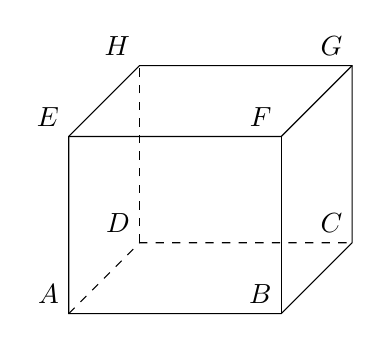
\begin{tikzpicture}[scale=.9]
\coordinate(A)at(0,0);\coordinate(B)at(3,0);\coordinate(D)at(1,1);\coordinate(C)at(4,1);
\coordinate(E)at(0,2.5);\coordinate(F)at(3,2.5);\coordinate(H)at(1,3.5);\coordinate(G)at(4,3.5);
\draw(A)--(B)--(C)--(G)--(H)--(E)--cycle;\draw(E)--(F)--(G);\draw(B)--(F);
\draw[dashed](A)--(D)--(C);\draw[dashed](D)--(H);
\foreach \p in {A,B,C,D,E,F,G,H}\node[above left]at(\p){$\p$};
\end{tikzpicture}
\end{center}
Dans le repère $(A;\overrightarrow{AB},\overrightarrow{AD},\overrightarrow{AE})$, $G=(1,1,1)$, le centre du cube est $(1/2,1/2,1/2)$ et $\overrightarrow{BH}=(-1,1,1)$.
Le dessin est une projection : des droites qui s'y croisent peuvent être disjointes dans l'espace.
\section{Positions relatives}
Deux droites peuvent être confondues, parallèles distinctes, sécantes ou non coplanaires (gauches). Deux plans sont confondus, parallèles distincts ou sécants suivant une droite. Une droite est contenue dans un plan, parallèle sans point commun, ou sécante en un point.
\begin{exemple}
Les droites $(t,0,0)$ et $(0,s,1)$ n'ont aucun point commun car leurs troisièmes coordonnées diffèrent. Leurs directions ne sont pas colinéaires : elles sont gauches.
Pour montrer $A,B,C,D$ coplanaires, avec $\overrightarrow{AB}$ et $\overrightarrow{AC}$ non colinéaires, chercher $s,t$ tels que $\overrightarrow{AD}=s\overrightarrow{AB}+t\overrightarrow{AC}$.
\end{exemple}
\begin{finchapitre}
\section{Utilité et suite du parcours}
La géométrie fournit des modèles concrets de liberté, de dimension et de sous-espace. En licence, on remplacera les flèches par des polynômes, des fonctions ou des suites sans changer la logique des combinaisons linéaires.
\begin{retenir}
Un plan exige deux directions non colinéaires ; une base de l'espace en exige trois non coplanaires. Un dessin seul ne décide pas une intersection.
\end{retenir}
\end{finchapitre}
\end{document}
